\subsection{Da MIP à matriz de atribuição de emissões}
\label{sec:derivacao}

A análise utiliza a matriz $A$ de coeficientes técnicos de insumos nacionais, a produção bruta $x$ e a demanda final por atividade $y$. Os índices $i$ e $j$ identificam atividades, e os vetores são colunas. Cada $A_{ij}$ indica o insumo de $i$ requerido por unidade monetária de produção de $j$. O balanço e a inversa de Leontief são
\begin{equation}
x=Ax+y=Ly,\qquad L=(I-A)^{-1}.
\label{eq:leontief}
\end{equation}
$L_{ij}$ reúne a produção de $i$ requerida direta e indiretamente por unidade de demanda final de $j$, sob coeficientes técnicos fixos \parencite{millerBlair2009}. A consistência de $A$ e $L$ e o balanço $Ly=x$ são conferidos considerando o arredondamento da fonte.

Seja $\varphi_i$ a intensidade direta de CO\textsubscript{2} por unidade de produção bruta de $i$, descrita na seção~\ref{sec:dados}. Organizando as intensidades em $\Phi=\operatorname{diag}(\varphi)$, obtém-se
\begin{equation}
C=\Phi L,\qquad C_{ij}=\varphi_iL_{ij}.
\label{eq:coeficientes-emissoes}
\end{equation}
Cada $C_{ij}$ expressa a emissão em $i$ por unidade monetária de demanda final de $j$, em Gg de CO\textsubscript{2} por milhão de reais \parencite{sanguinetAzzoni2024}.

Multiplicar cada coluna de $C$ pela demanda final efetiva fornece a matriz de atribuição:
\begin{equation}
F=C\widehat y=\Phi L\widehat y,\qquad F_{ij}=\varphi_iL_{ij}y_j,
\label{eq:matriz-atribuicao}
\end{equation}
em que $\widehat y=\operatorname{diag}(y)$. O elemento $F_{ij}$ representa a emissão ocorrida em $i$ e atribuída à demanda final dos produtos de $j$, incluindo requisitos diretos e indiretos. A matriz tem dimensão $67\times67$, em Gg de CO\textsubscript{2}, e conecta as contas pela produção e pela demanda \parencite{marques2012}. Seus elementos representam atribuições contábeis, não transações diretas nem transferências físicas de CO\textsubscript{2}.

\subsection{Atribuição pela produção e pela demanda}
\label{sec:atribuicoes}

A matriz $F$ permite organizar as mesmas emissões segundo a atividade em que ocorrem ou o produto final ao qual são atribuídas. A Figura~\ref{fig:exemplo-atribuicoes} ilustra essa distinção em uma economia de quatro atividades: Eletricidade, Agricultura, Alimentos e Restaurantes.

Na atribuição pela produção, somam-se as linhas de $F$, preservando a origem emissora:
\begin{equation}
c_i=\sum_jF_{ij}=\varphi_i x_i,\qquad c=F\mathbf{1}=\Phi x.
\label{eq:conta-producao}
\end{equation}
Aqui, $\mathbf{1}$ é um vetor-coluna de uns. No quadro (a), as emissões da geração elétrica são contabilizadas em Eletricidade, inclusive quando sua produção atende às outras atividades.

Na atribuição pela demanda, somam-se as colunas de $F$, preservando o setor do produto final:
\begin{equation}
u_j=\sum_iF_{ij}=y_j\sum_i\varphi_iL_{ij},\qquad u=F^\top\mathbf{1},
\label{eq:conta-demanda}
\end{equation}
em que $\top$ indica transposição. No quadro (b), a atribuição à demanda final de Restaurantes reúne suas emissões próprias e as de Eletricidade, Agricultura e Alimentos associadas ao atendimento dessa demanda. A produção é a mesma do quadro (a); muda sua atribuição.

O Sankey do quadro (c) conecta as duas contas: cada faixa representa $F_{ij}$, e as barras de origem e destino totalizam $c_i$ e $u_j$. A faixa entre Eletricidade e Restaurantes, por exemplo, corresponde à emissão da primeira atividade atribuída à demanda final da segunda. As setas superiores representam transações monetárias; as faixas representam atribuições de emissões. O total é preservado:
\begin{equation}
\mathbf{1}^\top c=\mathbf{1}^\top F\mathbf{1}=\mathbf{1}^\top u.
\label{eq:conservacao-emissoes}
\end{equation}

Para uma mesma atividade, a diferença entre as contas é o saldo das atribuições entre atividades distintas:
\begin{equation}
u_i-c_i=\sum_{j\ne i}F_{ji}-\sum_{j\ne i}F_{ij}.
\label{eq:saldo-atribuicao}
\end{equation}
A diagonal cancela no saldo, mas permanece nas contas completas. Um saldo pequeno pode resultar de grandes volumes atribuídos em sentidos opostos; por isso, é necessário examinar as relações que o compõem.

% Figura vetorial copiada sem edição de:
% C:/GitHub/Mestrado/0-Projeto de Dissertação/figura_economia/contabilidade_com_sankey.pdf
% SHA-256: 861F8B5C1FDEBE3C96B31D8BD96763C2829FA2AE72703160C83949E4ACD6BF29
\begin{figure}[p]
\centering
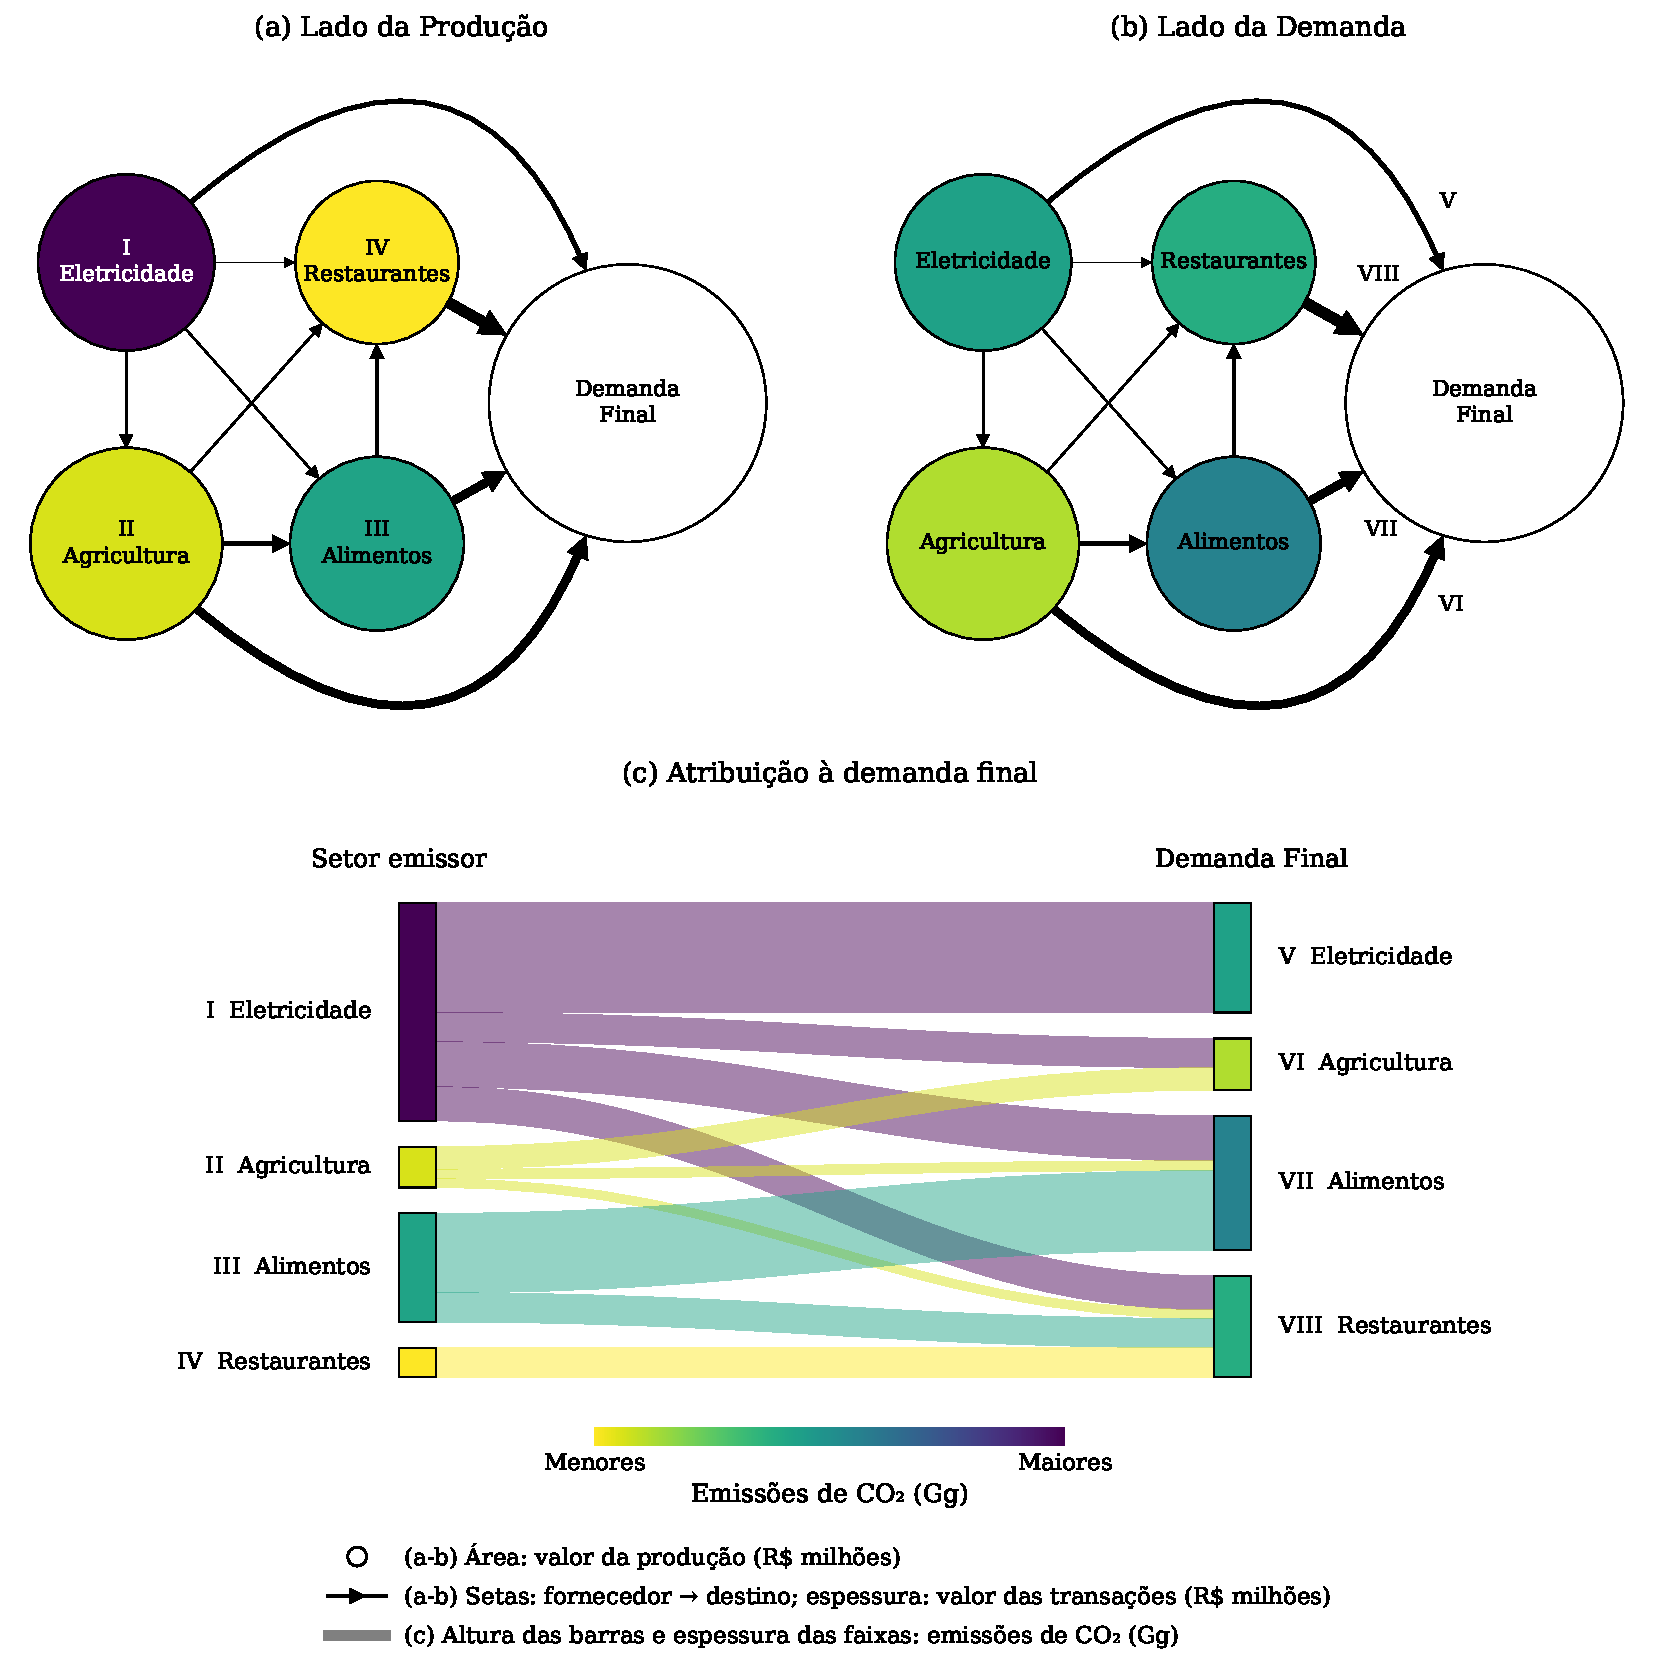
\includegraphics[width=\textwidth,height=0.76\textheight,keepaspectratio]{figuras/atribuicao_cadeia_alimentos.pdf}
\caption{Atribuição das emissões pela produção e pela demanda em uma economia ilustrativa.}
\label{fig:exemplo-atribuicoes}
\begin{minipage}{\textwidth}\footnotesize
Fonte: elaboração própria.

Nota: exemplo didático, sem representar estimativas nacionais dos quatro setores. Em (a--b), áreas e espessuras das setas expressam valores monetários; no nó Demanda Final, a área indica o valor recebido, incluindo exportações. As cores representam $c$ em (a) e $u$ em (b). Em (c), as barras à esquerda representam as origens emissoras (I--IV) e as barras à direita, os produtos finais (V--VIII). Suas alturas e as espessuras das faixas expressam emissões em Gg de CO\textsubscript{2}. Os três quadros compartilham a escala de cores.
\end{minipage}
\end{figure}
\clearpage
